\section{Projektplanung}\label{sec:projektplanung}

\subsection{Zieldefinition}\label{subsec:zieldefinition}
Das Ziel dieses Projekts ist die Entwicklung und Implementierung einer universellen Sammlerplattform, die es Benutzern ermöglicht, ihre Sammlungen digital zu verwalten, zu präsentieren und mit anderen zu teilen.
Diese Plattform soll benutzerfreundlich, flexibel und skalierbar sein, um eine breite Palette von Sammlerbedürfnissen abzudecken.

% Wir könnten hier sicherlich auch das Wording Meilensteine nutzen, finde ich besser als Teilergebnisse
\subsection{Teilergebnisse}\label{subsec:teilergebnisses}
Die Teilergebnisse lassen sich aus dem Konzept in ~\ref{subsec:Designphase} ableiten.
Grundlegende Teilergebnisse sind die Erstellung des Frontends, die Erstellung des Backends und die Einrichtung einer Datenbank.
Neben diesen Zielen, die sich aus der verwendeten Architektur ergeben, ist ein weiteres Teilergebnis das Hosting der Website und der Datenbank.
Für jedes Teilergebnis sind Voranalysen notwendig, da die Programmierung einer Webanwendung für das gesamte Team neu ist.
Als Ausgangspunkt für die Analyse diente GitHub Eduction, das mit dem Kurs Intro to Web Development einige Tools für die Entwicklung von Websites zur Verfügung stellt.
Die in der Analyse ausgewählten Tools sind in ~\ref{subsec:Tools} aufgelistet.

Die Teilergebnisse sind eng miteinander verknüpft.
Das Hosting der Website und der Datenbank sind von entscheidender Bedeutung.
Insbesondere das Backend ist ohne die Datenbank nur schwer zu entwickeln.
Das Hosting der Website ist wichtig, um die integrierten Funktionen direkt live testen zu können.
Die Entwicklung von Frontend, Backend und Datenbank ist eng miteinander verzahnt.
Frontend und Datenbank lassen sich separat einrichten, das Backend ist für die Kommunikation der beiden Bereiche unerlässlich.
Während die drei Bereiche einzelne Teilergebnisse darstellen, erfolgt der Großteil der Programmierung parallel.

Das Frontend ist alles, womit der Benutzer letztendlich auf der Website interagieren kann.
Beispiele hierfür sind die Login-Seite, die Ansicht der verschiedenen Sammlungen und die Seite zur Erstellung von Vorlagen.
Im Anhang finden sich Mockups, die während des anfänglichen Brainstormings der Projektidee entstanden sind.
Das Backend ist für die Kommunikation zwischen dem Frontend und der Datenbank verantwortlich.
Es soll die Daten aus der Datenbank an das Frontend zur Anzeige weiterleiten.
Außerdem soll es Änderungen an den Daten, die in der Benutzeroberfläche vorgenommen werden, an die Datenbank kommunizieren.
Dabei ist es wichtig, dass die Funktionen sicherstellen, dass die Datenbank dynamisch auf Basis der Benutzereingaben skaliert wird.
Die Logik der Website sollte in diesem Teil des Programms definiert werden.
Das Datenbanksystem ist der Ort, an dem Informationen über Benutzer und Sammlungen gespeichert werden.
Die Datenbankform der Sammlungsvorlagen wird hier gespeichert.
Es muss so konfiguriert sein, dass das dynamische Hinzufügen und Löschen ganzer Tabellen möglich ist.
% Vllt mal ein Mockup für ein Template erstellen

\subsection{Definitions of done}\label{subsec:definitions-of-done}

\setlist{nolistsep}
\newcolumntype{L}{>{\raggedright\arraybackslash}X}
\newcolumntype{R}{>{\raggedright\arraybackslash}X}


Im Rahmen des Projekts wurden die folgenden Definitions of Done festgelegt, um den erfolgreichen Abschluss der verschiedenen Projektaufgaben und -phasen sicherzustellen:

    \begin{tabularx}{\textwidth}{L R}
        \begin{enumerate}[left=0pt,label=\arabic*.]
            \small
            \item \textbf{Die Idee des Projektes ist erstellt:}
            \begin{itemize}[label=--]
                \item Eine klare und detaillierte Beschreibung des Projektziels und der Motivation liegt vor.
            \end{itemize}

            \item \textbf{Auswahl der genutzten Software- bzw. Projektwerkzeuge ist erfolgt:}
            \begin{itemize}[label=--]
                \item Alle notwendigen Software- und Projektmanagement-Tools sind ausgewählt und dokumentiert.
            \end{itemize}

            \item \textbf{Projektplanung ist angelegt:}
            \begin{itemize}[label=--]
                \item Ein detaillierter Projektplan mit Zeitplan, Meilensteinen und Ressourcenplanung ist erstellt.
                \item Der Projektplan ist mit dem Projektteam abgestimmt und genehmigt.
            \end{itemize}

            \item \textbf{Erstellung von Konzept und Projektplan (Abgabe 1) erfolgreich und genehmigt:}
            \begin{itemize}[label=--]
                \item Das Konzept und der Projektplan sind fertiggestellt und den entsprechenden Gremien oder Betreuern vorgelegt.
                \item Eine formelle Genehmigung oder Freigabe wurde erteilt.
            \end{itemize}

            \item \textbf{Anlegen der Projektumgebung mithilfe der Software- bzw. Projektwerkzeuge erfolgte:}
            \begin{itemize}[label=--]
                \item Die Projektumgebung ist vollständig eingerichtet, einschließlich aller erforderlichen Software- und Hardwarekomponenten.
                \item Alle Teammitglieder haben Zugang und die notwendige Schulung für die genutzten Werkzeuge erhalten.
            \end{itemize}

            \item \textbf{Backend-System ist implementiert:}
            \begin{itemize}[label=--]
                \item Das Backend-System ist vollständig entwickelt und funktionsfähig.
                \item Alle geplanten Funktionen und Schnittstellen sind implementiert und getestet.
            \end{itemize}



        \end{enumerate}
        &
        \begin{enumerate}[left=0pt,label=\arabic*.]
            \setcounter{enumi}{6}
            \small
            \item \textbf{Frontend-System ist implementiert:}
            \begin{itemize}[label=--]
                \item Das Frontend-System ist vollständig entwickelt und funktionsfähig, als auch benutzerfreundlich.
            \end{itemize}
            \item \textbf{Datenbanksystem ist implementiert:}
            \begin{itemize}[label=--]
                \item Die Datenbank ist eingerichtet, strukturiert und alle notwendigen Tabellen und Beziehungen sind vorhanden.
            \end{itemize}

            \item \textbf{Verknüpfung der drei Systeme erfolgte:}
            \begin{itemize}[label=--]
                \item Backend, Frontend und Datenbanksystem sind nahtlos integriert.
            \end{itemize}

            \item \textbf{Account-Erstellung und Benutzer-Login ist möglich:}
            \begin{itemize}[label=--]
                \item Nutzer können erfolgreich Accounts erstellen und sich in das System einloggen.
            \end{itemize}

            \item \textbf{Vorhandene „Sammlungen“-Templates können genutzt werden:}
            \begin{itemize}[label=--]
                \item Standard-Templates für Sammlungen sind verfügbar und können von den Benutzern angewendet werden.
                \item Diese Templates sind funktional und ansprechend gestaltet.
            \end{itemize}

            \item \textbf{Benutzer kann erfolgreich eigene Templates anlegen:}
            \begin{itemize}[label=--]
                \item Nutzer haben die Möglichkeit, eigene Templates für ihre Sammlungen zu erstellen und zu speichern.
            \end{itemize}
            \item \textbf{Benutzerrechte-Einstellungen sind passend:}
            \begin{itemize}[label=--]
                \item Benutzerrechte und -rollen sind definiert und korrekt implementiert.
                \item Die Plattform stellt sicher, dass Benutzer nur auf die ihnen zugewiesenen Bereiche und Funktionen zugreifen können.
            \end{itemize}
        \end{enumerate}
    \end{tabularx}


    \vspace{0.5cm}
    \begin{tabularx}{\textwidth}{L R}
        \begin{enumerate}[left=0pt,label=\arabic*.]
            \setcounter{enumi}{13}
            \small

            \item \textbf{Alle notwendigen Tests erfolgreich:}
            \begin{itemize}[label=--]
                \item Alle geplanten Tests (Unit-Tests, Integrationstests, Systemtests, Usability-Tests) sind abgeschlossen.
                \item Die Testergebnisse sind dokumentiert und alle kritischen Fehler sind behoben.
            \end{itemize}

            \item \textbf{Projektdokumentation ist erstellt:}
            \begin{itemize}[label=--]
                \item Eine vollständige und detaillierte Dokumentation des Projekts ist vorhanden.
            \end{itemize}

        \end{enumerate}
        &
        \begin{enumerate}[left=0pt,label=\arabic*.]
            \setcounter{enumi}{16}
            \small
            \item \textbf{Präsentation fertiggestellt:}
            \begin{itemize}[label=--]
                \item Eine umfassende Präsentation ist vorbereitet, die alle wichtigen Funktionen und Vorteile der Plattform darstellt.
            \end{itemize}

            \item \textbf{Projektbericht + Präsentation (Abgabe 2):}
            \begin{itemize}[label=--]
                \item Der abschließende Projektbericht ist fertiggestellt und eingereicht.
                \item Die Präsentation wurde erfolgreich fertiggestellt und durchgeführt.
            \end{itemize}
        \end{enumerate}
    \end{tabularx}

\newpage


\begin{tabularx}{\textwidth}{L R}
    \begin{enumerate}[left=0pt,label=\arabic*.]
        \setcounter{enumi}{11}
        \small
        \item \textbf{Benutzer kann erfolgreich eigene Templates anlegen:}
        \begin{itemize}[label=--]
            \item Nutzer haben die Möglichkeit, eigene Templates für ihre Sammlungen zu erstellen und zu speichern.
        \end{itemize}

        \item \textbf{Benutzerrechte-Einstellungen sind passend:}
        \begin{itemize}[label=--]
            \item Benutzerrechte und -rollen sind definiert und korrekt implementiert.
            \item Die Plattform stellt sicher, dass Benutzer nur auf die ihnen zugewiesenen Bereiche und Funktionen zugreifen können.
        \end{itemize}

        \item \textbf{Alle notwendigen Tests erfolgreich:}
        \begin{itemize}[label=--]
            \item Alle geplanten Tests (Unit-Tests, Integrationstests, Systemtests, Usability-Tests) sind abgeschlossen.
            \item Die Testergebnisse sind dokumentiert und alle kritischen Fehler sind behoben.
        \end{itemize}

        \item \textbf{Projektdokumentation ist erstellt:}
        \begin{itemize}[label=--]
            \item Eine vollständige und detaillierte Dokumentation des Projekts ist vorhanden.
        \end{itemize}

        \item \textbf{Produktpräsentation fertiggestellt:}
        \begin{itemize}[label=--]
            \item Eine umfassende Produktpräsentation ist vorbereitet, die alle wichtigen Funktionen und Vorteile der Plattform darstellt.
        \end{itemize}

        \item \textbf{Projektbericht + Präsentation (Abgabe 2):}
        \begin{itemize}[label=--]
            \item Der abschließende Projektbericht ist fertiggestellt und eingereicht.
            \item Die Präsentation wurde erfolgreich fertiggestellt und durchgeführt.
        \end{itemize}
    \end{enumerate}
    &
\end{tabularx}


\subsection{Projektstrukturplan}\label{subsec:projektstrukturplan}
Lorenz ipsum dolor sit amet, consetetur sadipscing elitr, sed diam nonumy eirmod tempor invidunt ut labore et dolore magna aliquyam erat, sed diam voluptua.
At vero eos et accusam et justo duo dolores et ea rebum.
Stet clita kasd gubergren, no sea takimata sanctus est Lorem ipsum dolor sit amet.
Lorenz ipsum dolor sit amet, consetetur sadipscing elitr, sed diam nonumy eirmod tempor invidunt ut labore et dolore magna aliquyam erat, sed diam voluptua.
At vero eos et accusam et justo duo dolores et ea rebum.
Stet clita kasd gubergren, no sea takimata sanctus est Lorem ipsum dolor sit amet.
Lorenz ipsum dolor sit amet, consetetur sadipscing elitr, sed diam nonumy eirmod tempor invidunt ut labore et dolore magna aliquyam erat, sed diam voluptua.
At vero eos et accusam et justo duo dolores et ea rebum.
Stet clita kasd gubergren, no sea takimata sanctus est Lorem ipsum dolor sit amet.

\begin{figure}[H]
    \centering
    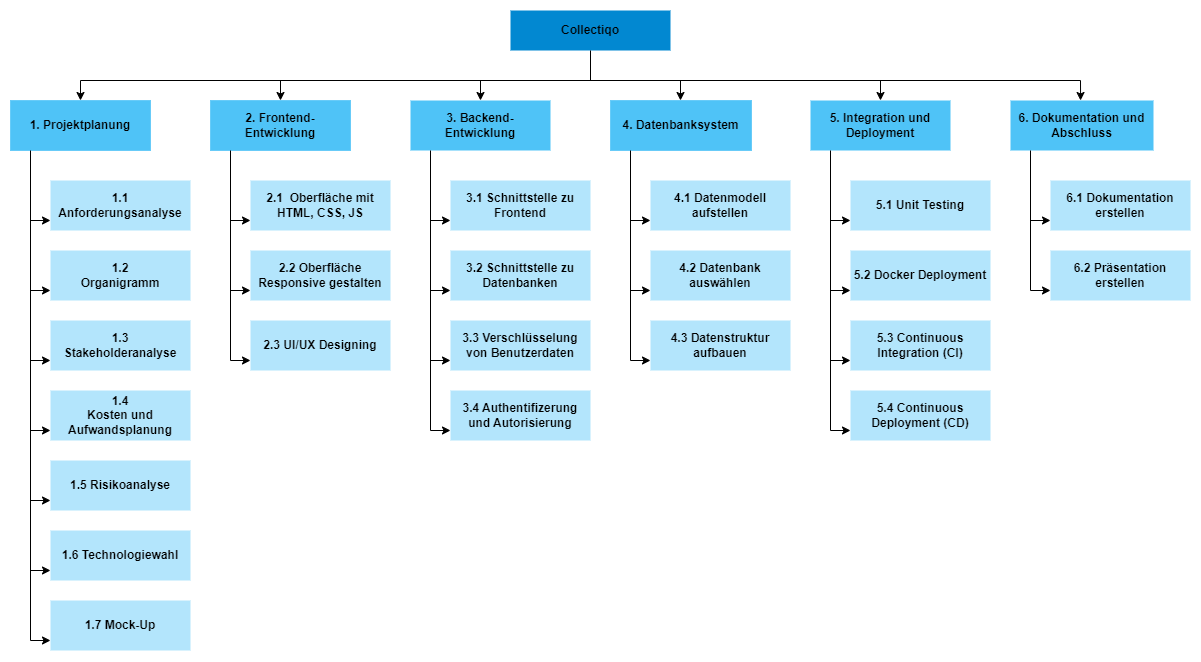
\includegraphics[width=1.0\textwidth]{psp}
    \caption{Projektstrukturplan}\label{fig:projektstrukturplan}
\end{figure}